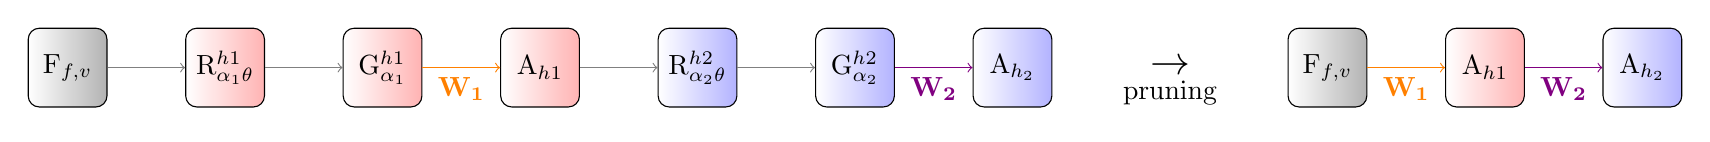
\begin{tikzpicture}
[transform shape,rotate=0, node distance=2.0cm and 2.0cm,
ar/.style={->,>=latex},
mynode/.style={
  draw, scale = 1.0,  minimum size=1cm, rounded corners,left color=white,
  minimum height=1cm,
  align=center
  }
]

\tikzstyle{neuron}  =  [rectangle, draw, scale = 1.0,  minimum size=1cm]
\tikzstyle{treenode}  =  [mynode, right color=black!30!white]
\tikzstyle{recnode}  =  [mynode, right color=magenta!30!white]
\tikzstyle{qnode}  =  [mynode, right color=blue!30!white]
\tikzstyle{grbond}  =  [mynode, right color=black!30!white]
\tikzstyle{gratom}  =  [mynode]
\tikzstyle{grgroup} =  [mynode, right color=brown!30!white]
\tikzstyle{grexpl}  =  [mynode, right color=violet!30!white]
\tikzstyle{edgenode}  =  [thin, draw=black, align=center,fill=white,font=\small]


\node[treenode] (f1) {F$_{f,v}$};
\node[recnode,right color=red!30!white] (r1) [right of=f1] {R$_{\alpha_1\theta}^{h1}$};
\node[recnode,right color=red!30!white] (g1) [right of=r1] {G$_{\alpha_1}^{h1}$};
\node[recnode,right color=red!30!white] (a1) [right of=g1] {A$_{h1}$};

\node[recnode,right color=blue!30!white] (r2) [right of=a1] {R$_{\alpha_2\theta}^{h2}$};
\node[recnode,right color=blue!30!white] (g2) [right of=r2] {G$_{\alpha_2}^{h2}$};
\node[qnode,right color=blue!30!white] (a2) [right of=g2] {A$_{h_2}$};

%edges

\draw[gray,->] (f1) -> node[gray, below] {} (r1);
\draw[gray,->] (r1) -> node[gray, below] {} (g1);
\draw[orange,->] (g1) -> node[ below] {$\mathbf{W_1}$} (a1);

\draw[gray,->] (a1) -> node[gray, below] {} (r2);
\draw[gray,->] (r2) -> node[gray, below] {} (g2);
\draw[violet,->] (g2) -> node[ below] {$\mathbf{W_2}$} (a2);


\node[mynode, draw=white, label={[xshift=0.0cm, yshift=-1.1cm]{pruning}}] (prune) [right of=a2] {\Large $\rightarrow$};


% pruned
\node[treenode] (ff1) [right of=prune] {F$_{f,v}$};
\node[recnode,right color=red!30!white] (aa1) [right of=ff1] {A$_{h1}$};
\node[qnode] (aa2) [right of=aa1] {A$_{h_2}$};

\draw[orange,->] (ff1) -> node[below] {$\mathbf{W_1}$} (aa1);
\draw[violet,->] (aa1) -> node[below] {$\mathbf{W_2}$} (aa2);

\end{tikzpicture}